
\subsection[Sp(n,R)]{$\mathrm{Sp}(n,\R) \sim C_n, n \geq 2$}

\subsubsection{Root system data}

\[ \alpha_i = \epsilon_i - \epsilon_{i+1}, i< n,a_n = 2\epsilon_n, \quad \omega_i=\epsilon_1+\cdots+\epsilon_i\]
\begin{align*}
 \roots &= \{\pm \epsilon_i \pm \epsilon_j | i,j = 1,\ldots, n \}\setminus\{0\}\\
 \roots_c^+ &= \{ \epsilon_i-\epsilon_j | 1\leq i < j \leq  n\}\\
 \roots_n^+ &= \{ \epsilon_i + \epsilon_j | 1 \leq i \leq  j \leq n \}
\end{align*}
\[\beta = 2\epsilon_1,\quad \rho = (n,\ldots ,1),\quad \zeta = (1,1,\ldots,1)\]
\inserttikzfigure{diagrams/dynkin_Cn_n.tikz}{Marked Dynkin diagram of $\mathrm{Sp}(n,\R)$}

The reduction points of unitarizable highest weight modules are the following integral translated cones $\lambda_a + C_a$:
Let $a=(Q,R,l)$, $R=\mathrm{Sp}(r,\R)$ and $1\leq l \leq r \leq n$. Then
\[
 C_a = \{ a_r\omega_r + \cdots + a_n\omega_n \,|\, a_n=-(a_r+\cdots + a_{n-1}) \}
\]
and
\begin{gather*}
  \lambda_a = \omega_q + \omega_r - (2+n-\frac{1}{2}(r+q-l+1))\omega_n\\
  \mu_a= \omega_{q-l} + \omega_{r-l} - (2+n-\frac{1}{2}(r+q-l+1))\omega_n\\
   1\leq q\leq r\leq n,\quad 1\leq l \leq q\\
   Q(\lambda_a) = \mathrm{Sp}(q,\R),\quad R(\lambda_a)= \mathrm{Sp}(r,\R)
\end{gather*}

\subsubsection{Nilpotent cohomology in detail}

Scalar products of $\rho$ with noncompact roots
\begin{align*}
 (\epsilon_i - \epsilon_j, \rho ) & = n-i+1 - (n-j+1) = j - i \\
 (\epsilon_i + \epsilon_j, \rho ) & = n-i+1 + (n-j+1) = 2n+2-i-j.
\end{align*}


The $i$th coordinate of $\lambda$ with respect to the $\epsilon$-basis is
\[
 (\epsilon_i, \lambda) = \begin{cases}
                          2+ \frac{1}{2}(r+q-l+1) - n -2, & 1\leq i \leq q \\
                          1 + \frac{1}{2}(r+q-l+1) - n -2,  & q < i \leq r \\
                          \frac{1}{2}(r+q-l+1) - n -2,  & r < i.
                         \end{cases}
\]
Computation of $(\epsilon_i - \epsilon_j, \lambda + \rho)$ for $j > i$ leads to the following table
\begin{center}
\begin{tabular}{C|CCC}
                  & 1 < j \leq q & q < j \leq r & r < j \leq n \\[2pt]\hline
   1\leq i \leq q & j - i        & 1+j-i        & 2+j-i        \\
  q < i \leq r    &              & j-i		& 1+j-i        \\
  r < i \leq n	  & 		 & 		& j-i	
\end{tabular}
\end{center}
and  scalar products of the remaining positive roots $\epsilon_i + \epsilon_j$, $j\geq i$ are
\begin{center}
\begin{tabular}{C|CCC}
                  & 1 < j \leq q & q < j \leq r & r < j \leq n \\[2pt]\hline
   1\leq i \leq q & 3+m-i-j      & 2 + m -i-j   & 1 + m  -i-j      \\
  q < i \leq r    &              & 1 + m-i-j	& m    -i-j    \\
  r < i \leq n	  & 		 & 		& m-1-i-j
\end{tabular}
\end{center}
where
\[
 m = r+q-l.
\]
We see again that only noncompact roots can be orthogonal to $\lambda+\rho$ in accordance with the lemma \ref{lem:singular_are_noncompact}. If a positive noncompact root $\epsilon_i + \epsilon_j$ belongs to $\Psi^+_\lambda$, then
\begin{enumerate}
  \item $1\leq i \leq q$
    \begin{enumerate}
      \item $1 \leq j \leq q$: \[ 3+r-l \leq i \leq \min \left\{ q, \frac{3+m}{2} \right \}\]
      \item $q < j \leq r$: \[ 2+q-l \leq i \leq \min \{ 1+r-l, q \}  \]
      \item $r < j \leq n$: \[ \max \{ 1, 1+m-n \} \leq i \leq q-l  \]
    \end{enumerate}
  \item $q <  i \leq r$
    \begin{enumerate}
      \item $q < j \leq r$: \[  1+q \leq i \leq \frac{1+m}{2} \]
      \item $r < j \leq n$: \[ m-n \leq i < q-l \]
    \end{enumerate}
  \item $r < i \leq n$, \quad $r < j \leq n$: \[ \max \{ r+1,  m-n-1 \} \leq i \leq \frac{m-1}{2}. \]
\end{enumerate}
The set of indices 2a is empty, because $q-l < q$; similarly the third set is empty since $r+1 > \frac{m-1}{2}$.

A singular long root exists if and only if
\[
  m \text{ is odd and } (3+r \leq q+l \text{ or } q+l < 1+r)
\]
or alternatively a singular root doesn't exist if and only if
\[
 m \text{ is even or } m \text{ is odd and either } q+l = 2+r \text{ or } q+l = 1+r.
\]


Two positive noncompact roots are orthogonal if and only if the intersection of their indices is empty, i.e.
\[
 (\epsilon_i + \epsilon_j,\epsilon_k + \epsilon_l) = 0 \Longleftrightarrow \{i,j\} \cap \{k,l\} = \emptyset.
\]


\begin{figure}[H]
  \centering 
  \resizebox{\textwidth}{!}{%
	\begin{tikzpicture}[>=latex,line join=bevel,]
%%
\node (alpha3+2*alpha4+alpha5) at (89bp,268bp) [draw,draw=none] {$\alpha_{3} + 2\alpha_{4} + \alpha_{5}$};
  \node (alpha1+alpha2+2*alpha3+2*alpha4+alpha5) at (208bp,112bp) [draw,draw=none] {$\alpha_{1} + \alpha_{2} + 2\alpha_{3} + 2\alpha_{4} + \alpha_{5}$};
  \node (alpha5) at (125bp,420bp) [draw,draw=none] {$\alpha_{5}$};
  \node (2*alpha2+2*alpha3+2*alpha4+alpha5) at (79bp,112bp) [draw,draw=none] {$2\alpha_{2} + 2\alpha_{3} + 2\alpha_{4} + \alpha_{5}$};
  \node (alpha1+alpha2+alpha3+2*alpha4+alpha5) at (208bp,164bp) [draw,draw=none] {$\alpha_{1} + \alpha_{2} + \alpha_{3} + 2\alpha_{4} + \alpha_{5}$};
  \node (2*alpha1+2*alpha2+2*alpha3+2*alpha4+alpha5) at (143bp,8bp) [draw,draw=none] {$2\alpha_{1} + 2\alpha_{2} + 2\alpha_{3} + 2\alpha_{4} + \alpha_{5}$};
  \node (alpha2+alpha3+2*alpha4+alpha5) at (137bp,216bp) [draw,draw=none] {$\alpha_{2} + \alpha_{3} + 2\alpha_{4} + \alpha_{5}$};
  \node (alpha2+alpha3+alpha4+alpha5) at (185bp,268bp) [draw,draw=none] {$\alpha_{2} + \alpha_{3} + \alpha_{4} + \alpha_{5}$};
  \node (alpha4+alpha5) at (125bp,371bp) [draw,draw=none] {$\alpha_{4} + \alpha_{5}$};
  \node (2*alpha3+2*alpha4+alpha5) at (36bp,216bp) [draw,draw=none] {$2\alpha_{3} + 2\alpha_{4} + \alpha_{5}$};
  \node (alpha1+2*alpha2+2*alpha3+2*alpha4+alpha5) at (143bp,60bp) [draw,draw=none] {$\alpha_{1} + 2\alpha_{2} + 2\alpha_{3} + 2\alpha_{4} + \alpha_{5}$};
  \node (alpha2+2*alpha3+2*alpha4+alpha5) at (81bp,164bp) [draw,draw=none] {$\alpha_{2} + 2\alpha_{3} + 2\alpha_{4} + \alpha_{5}$};
  \node (alpha1+alpha2+alpha3+alpha4+alpha5) at (256bp,216bp) [draw,draw=none] {$\alpha_{1} + \alpha_{2} + \alpha_{3} + \alpha_{4} + \alpha_{5}$};
  \node (2*alpha4+alpha5) at (89bp,320bp) [draw,draw=none] {$2\alpha_{4} + \alpha_{5}$};
  \node (alpha3+alpha4+alpha5) at (162bp,320bp) [draw,draw=none] {$\alpha_{3} + \alpha_{4} + \alpha_{5}$};
  \draw [black,->] (alpha2+2*alpha3+2*alpha4+alpha5) ..controls (119.09bp,148bp) and (156.76bp,133.17bp)  .. (alpha1+alpha2+2*alpha3+2*alpha4+alpha5);
  \draw [black,->] (alpha3+2*alpha4+alpha5) ..controls (74.101bp,252.94bp) and (60.793bp,240.39bp)  .. (2*alpha3+2*alpha4+alpha5);
  \draw [black,->] (alpha2+alpha3+alpha4+alpha5) ..controls (204.88bp,253bp) and (224.54bp,239.16bp)  .. (alpha1+alpha2+alpha3+alpha4+alpha5);
  \draw [black,->] (alpha3+alpha4+alpha5) ..controls (168.06bp,305.82bp) and (173.5bp,293.99bp)  .. (alpha2+alpha3+alpha4+alpha5);
  \draw [black,->] (alpha4+alpha5) ..controls (115.46bp,357.02bp) and (106.83bp,345.27bp)  .. (2*alpha4+alpha5);
  \draw [black,->] (alpha5) ..controls (125bp,407.84bp) and (125bp,397.19bp)  .. (alpha4+alpha5);
  \draw [black,->] (alpha1+alpha2+alpha3+2*alpha4+alpha5) ..controls (208bp,149.76bp) and (208bp,139.06bp)  .. (alpha1+alpha2+2*alpha3+2*alpha4+alpha5);
  \draw [black,->] (alpha3+alpha4+alpha5) ..controls (141.7bp,305.09bp) and (121.85bp,291.5bp)  .. (alpha3+2*alpha4+alpha5);
  \draw [black,->] (alpha1+alpha2+alpha3+alpha4+alpha5) ..controls (243.07bp,201.53bp) and (231.06bp,189.02bp)  .. (alpha1+alpha2+alpha3+2*alpha4+alpha5);
  \draw [black,->] (alpha4+alpha5) ..controls (134.92bp,356.86bp) and (144.07bp,344.75bp)  .. (alpha3+alpha4+alpha5);
  \draw [black,->] (2*alpha3+2*alpha4+alpha5) ..controls (48.516bp,201.09bp) and (59.504bp,188.88bp)  .. (alpha2+2*alpha3+2*alpha4+alpha5);
  \draw [black,->] (alpha3+2*alpha4+alpha5) ..controls (102.42bp,253.02bp) and (114.31bp,240.64bp)  .. (alpha2+alpha3+2*alpha4+alpha5);
  \draw [black,->] (2*alpha2+2*alpha3+2*alpha4+alpha5) ..controls (97.182bp,96.795bp) and (113.7bp,83.89bp)  .. (alpha1+2*alpha2+2*alpha3+2*alpha4+alpha5);
  \draw [black,->] (alpha1+2*alpha2+2*alpha3+2*alpha4+alpha5) ..controls (143bp,45.763bp) and (143bp,35.065bp)  .. (2*alpha1+2*alpha2+2*alpha3+2*alpha4+alpha5);
  \draw [black,->] (2*alpha4+alpha5) ..controls (89bp,305.76bp) and (89bp,295.06bp)  .. (alpha3+2*alpha4+alpha5);
  \draw [black,->] (alpha2+2*alpha3+2*alpha4+alpha5) ..controls (80.471bp,149.76bp) and (80.043bp,139.06bp)  .. (2*alpha2+2*alpha3+2*alpha4+alpha5);
  \draw [black,->] (alpha1+alpha2+2*alpha3+2*alpha4+alpha5) ..controls (189.44bp,96.721bp) and (172.43bp,83.639bp)  .. (alpha1+2*alpha2+2*alpha3+2*alpha4+alpha5);
  \draw [black,->] (alpha2+alpha3+2*alpha4+alpha5) ..controls (157.38bp,200.65bp) and (176.21bp,187.39bp)  .. (alpha1+alpha2+alpha3+2*alpha4+alpha5);
  \draw [black,->] (alpha2+alpha3+2*alpha4+alpha5) ..controls (121.17bp,200.87bp) and (106.92bp,188.14bp)  .. (alpha2+2*alpha3+2*alpha4+alpha5);
  \draw [black,->] (alpha2+alpha3+alpha4+alpha5) ..controls (172.07bp,253.53bp) and (160.06bp,241.02bp)  .. (alpha2+alpha3+2*alpha4+alpha5);
%
\end{tikzpicture}
	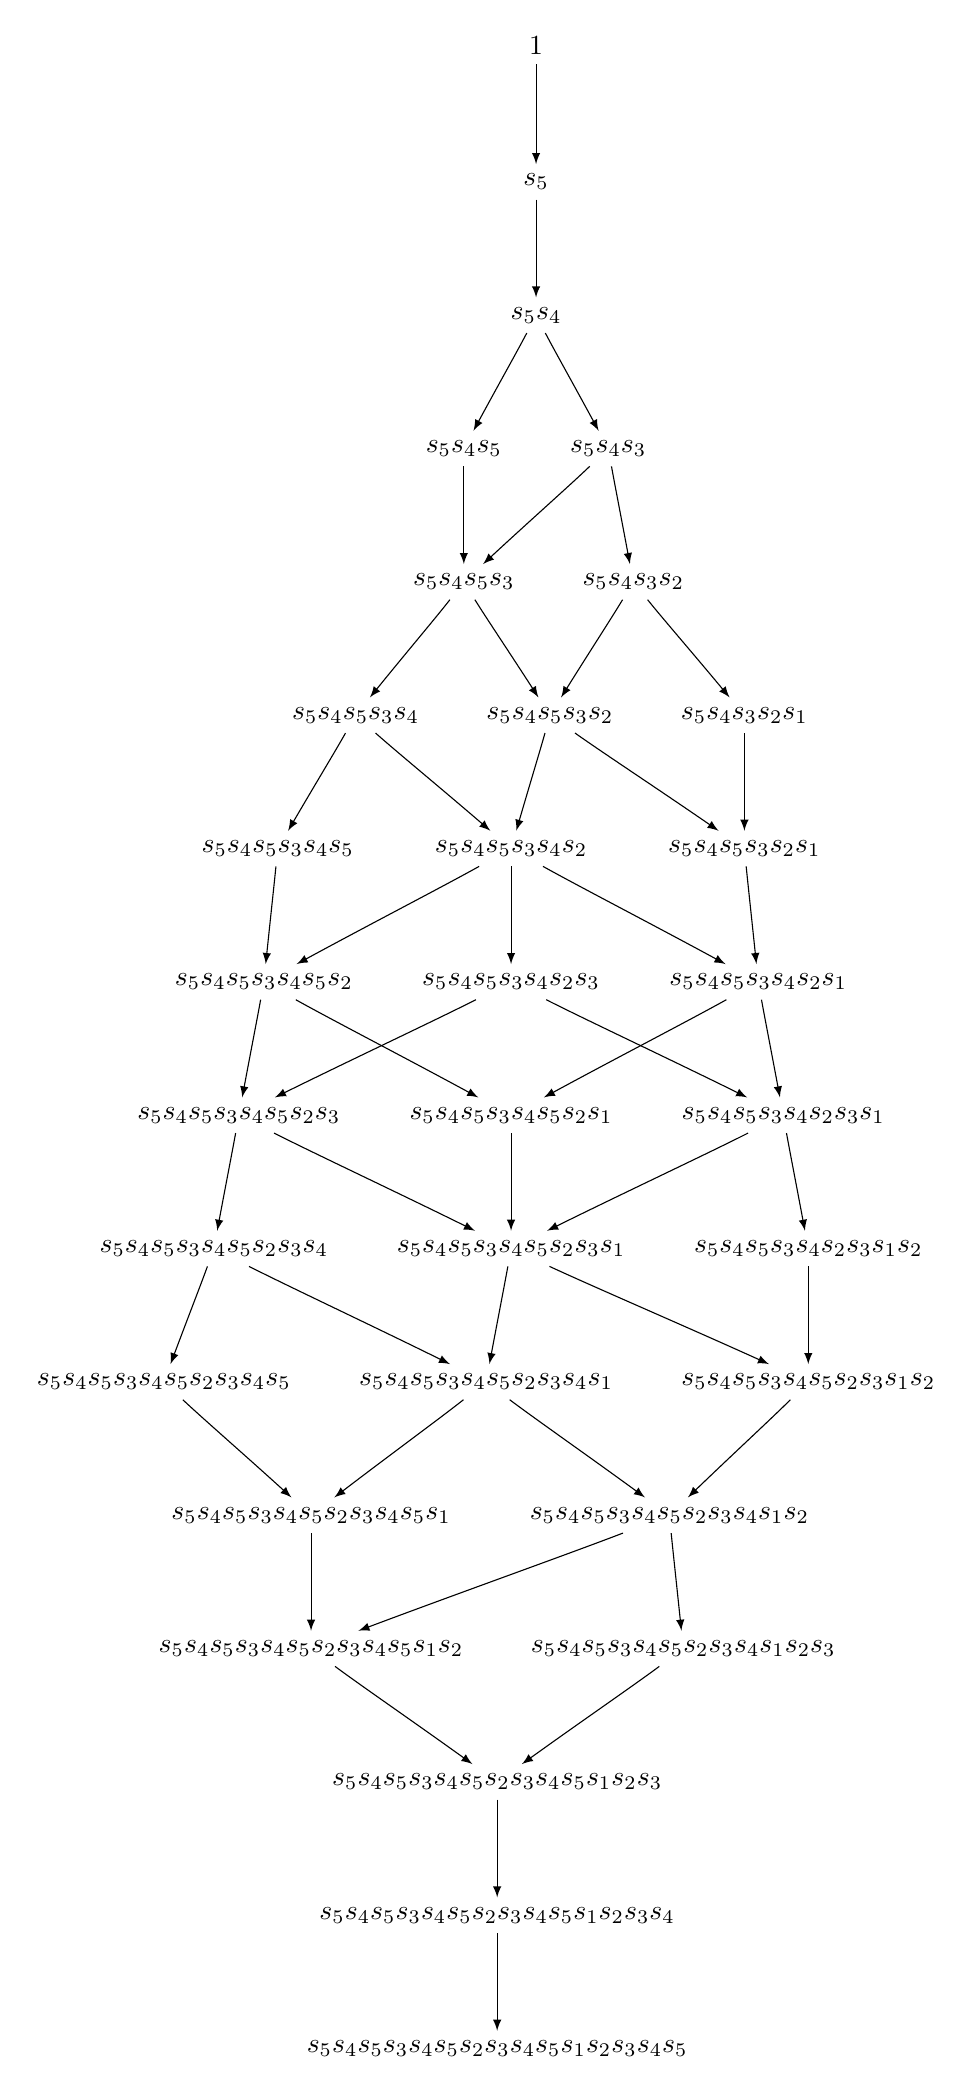
\begin{tikzpicture}[>=latex,line join=bevel,]
%%
\node (s5*s4*s5*s3*s4*s5*s2*s1) at (174bp,342bp) [draw,draw=none] {$s_{5}s_{4}s_{5}s_{3}s_{4}s_{5}s_{2}s_{1}$};
  \node (s5*s4*s5*s3*s4*s5*s2*s3*s4*s5*s1*s2) at (102bp,150bp) [draw,draw=none] {$s_{5}s_{4}s_{5}s_{3}s_{4}s_{5}s_{2}s_{3}s_{4}s_{5}s_{1}s_{2}$};
  \node (s5*s4*s5*s3*s4*s5*s2*s3*s4*s5*s1*s2*s3*s4*s5) at (169bp,6bp) [draw,draw=none] {$s_{5}s_{4}s_{5}s_{3}s_{4}s_{5}s_{2}s_{3}s_{4}s_{5}s_{1}s_{2}s_{3}s_{4}s_{5}$};
  \node (s5*s4*s5*s3*s4*s5*s2*s3*s4*s5*s1*s2*s3) at (169bp,102bp) [draw,draw=none] {$s_{5}s_{4}s_{5}s_{3}s_{4}s_{5}s_{2}s_{3}s_{4}s_{5}s_{1}s_{2}s_{3}$};
  \node (s5*s4) at (183bp,630bp) [draw,draw=none] {$s_{5}s_{4}$};
  \node (1) at (183bp,727bp) [draw,draw=none] {$1$};
  \node (s5*s4*s5*s3*s4*s5*s2*s3*s4) at (67bp,294bp) [draw,draw=none] {$s_{5}s_{4}s_{5}s_{3}s_{4}s_{5}s_{2}s_{3}s_{4}$};
  \node (s5*s4*s5*s3*s4*s5*s2*s3*s4*s5*s1*s2*s3*s4) at (169bp,54bp) [draw,draw=none] {$s_{5}s_{4}s_{5}s_{3}s_{4}s_{5}s_{2}s_{3}s_{4}s_{5}s_{1}s_{2}s_{3}s_{4}$};
  \node (s5*s4*s5*s3*s4*s5*s2*s3*s4*s1*s2*s3) at (236bp,150bp) [draw,draw=none] {$s_{5}s_{4}s_{5}s_{3}s_{4}s_{5}s_{2}s_{3}s_{4}s_{1}s_{2}s_{3}$};
  \node (s5*s4*s5*s3*s4*s5*s2*s3*s1) at (174bp,294bp) [draw,draw=none] {$s_{5}s_{4}s_{5}s_{3}s_{4}s_{5}s_{2}s_{3}s_{1}$};
  \node (s5) at (183bp,678bp) [draw,draw=none] {$s_{5}$};
  \node (s5*s4*s5*s3*s4*s2*s3*s1) at (272bp,342bp) [draw,draw=none] {$s_{5}s_{4}s_{5}s_{3}s_{4}s_{2}s_{3}s_{1}$};
  \node (s5*s4*s5*s3*s4*s5*s2*s3*s4*s1) at (165bp,246bp) [draw,draw=none] {$s_{5}s_{4}s_{5}s_{3}s_{4}s_{5}s_{2}s_{3}s_{4}s_{1}$};
  \node (s5*s4*s5*s3*s4*s5*s2*s3*s4*s5) at (49bp,246bp) [draw,draw=none] {$s_{5}s_{4}s_{5}s_{3}s_{4}s_{5}s_{2}s_{3}s_{4}s_{5}$};
  \node (s5*s4*s5*s3*s4*s5*s2*s3) at (76bp,342bp) [draw,draw=none] {$s_{5}s_{4}s_{5}s_{3}s_{4}s_{5}s_{2}s_{3}$};
  \node (s5*s4*s3*s2*s1) at (258bp,486bp) [draw,draw=none] {$s_{5}s_{4}s_{3}s_{2}s_{1}$};
  \node (s5*s4*s5*s3*s4*s5*s2*s3*s1*s2) at (281bp,246bp) [draw,draw=none] {$s_{5}s_{4}s_{5}s_{3}s_{4}s_{5}s_{2}s_{3}s_{1}s_{2}$};
  \node (s5*s4*s5*s3*s4*s5*s2) at (85bp,390bp) [draw,draw=none] {$s_{5}s_{4}s_{5}s_{3}s_{4}s_{5}s_{2}$};
  \node (s5*s4*s5*s3*s4*s2*s3*s1*s2) at (281bp,294bp) [draw,draw=none] {$s_{5}s_{4}s_{5}s_{3}s_{4}s_{2}s_{3}s_{1}s_{2}$};
  \node (s5*s4*s5*s3*s4*s2) at (174bp,438bp) [draw,draw=none] {$s_{5}s_{4}s_{5}s_{3}s_{4}s_{2}$};
  \node (s5*s4*s5*s3*s4*s5) at (90bp,438bp) [draw,draw=none] {$s_{5}s_{4}s_{5}s_{3}s_{4}s_{5}$};
  \node (s5*s4*s5*s3) at (157bp,534bp) [draw,draw=none] {$s_{5}s_{4}s_{5}s_{3}$};
  \node (s5*s4*s5*s3*s2) at (188bp,486bp) [draw,draw=none] {$s_{5}s_{4}s_{5}s_{3}s_{2}$};
  \node (s5*s4*s5*s3*s4*s5*s2*s3*s4*s1*s2) at (231bp,198bp) [draw,draw=none] {$s_{5}s_{4}s_{5}s_{3}s_{4}s_{5}s_{2}s_{3}s_{4}s_{1}s_{2}$};
  \node (s5*s4*s3*s2) at (218bp,534bp) [draw,draw=none] {$s_{5}s_{4}s_{3}s_{2}$};
  \node (s5*s4*s5*s3*s2*s1) at (258bp,438bp) [draw,draw=none] {$s_{5}s_{4}s_{5}s_{3}s_{2}s_{1}$};
  \node (s5*s4*s3) at (209bp,582bp) [draw,draw=none] {$s_{5}s_{4}s_{3}$};
  \node (s5*s4*s5*s3*s4) at (118bp,486bp) [draw,draw=none] {$s_{5}s_{4}s_{5}s_{3}s_{4}$};
  \node (s5*s4*s5) at (157bp,582bp) [draw,draw=none] {$s_{5}s_{4}s_{5}$};
  \node (s5*s4*s5*s3*s4*s5*s2*s3*s4*s5*s1) at (102bp,198bp) [draw,draw=none] {$s_{5}s_{4}s_{5}s_{3}s_{4}s_{5}s_{2}s_{3}s_{4}s_{5}s_{1}$};
  \node (s5*s4*s5*s3*s4*s2*s1) at (263bp,390bp) [draw,draw=none] {$s_{5}s_{4}s_{5}s_{3}s_{4}s_{2}s_{1}$};
  \node (s5*s4*s5*s3*s4*s2*s3) at (174bp,390bp) [draw,draw=none] {$s_{5}s_{4}s_{5}s_{3}s_{4}s_{2}s_{3}$};
  \draw [black,->] (s5*s4*s5*s3*s4*s5*s2*s3*s4*s1*s2) ..controls (194.81bp,184.1bp) and (152.73bp,169.09bp)  .. (s5*s4*s5*s3*s4*s5*s2*s3*s4*s5*s1*s2);
  \draw [black,->] (s5*s4*s5*s3*s4*s5*s2*s3*s4*s1) ..controls (147.99bp,232.58bp) and (130.3bp,219.66bp)  .. (s5*s4*s5*s3*s4*s5*s2*s3*s4*s5*s1);
  \draw [black,->] (s5*s4*s5*s3*s4*s2*s1) ..controls (238.63bp,376.41bp) and (211.29bp,362.27bp)  .. (s5*s4*s5*s3*s4*s5*s2*s1);
  \draw [black,->] (s5*s4*s5*s3*s4*s2) ..controls (198.37bp,424.41bp) and (225.71bp,410.27bp)  .. (s5*s4*s5*s3*s4*s2*s1);
  \draw [black,->] (s5*s4*s5*s3*s4*s2*s3*s1) ..controls (274.24bp,329.55bp) and (276.29bp,319.07bp)  .. (s5*s4*s5*s3*s4*s2*s3*s1*s2);
  \draw [black,->] (s5*s4*s5*s3*s4*s5*s2*s3*s4*s5*s1*s2*s3) ..controls (169bp,89.554bp) and (169bp,79.067bp)  .. (s5*s4*s5*s3*s4*s5*s2*s3*s4*s5*s1*s2*s3*s4);
  \draw [black,->] (s5*s4) ..controls (176.37bp,617.28bp) and (170.07bp,606.12bp)  .. (s5*s4*s5);
  \draw [black,->] (s5*s4*s5*s3*s4*s5*s2*s3*s4*s5*s1*s2) ..controls (119.83bp,136.76bp) and (139.03bp,123.57bp)  .. (s5*s4*s5*s3*s4*s5*s2*s3*s4*s5*s1*s2*s3);
  \draw [black,->] (s5*s4*s5*s3*s4*s5*s2*s3*s1*s2) ..controls (267.73bp,232.79bp) and (254.27bp,220.41bp)  .. (s5*s4*s5*s3*s4*s5*s2*s3*s4*s1*s2);
  \draw [black,->] (s5*s4*s5*s3) ..controls (164.99bp,521.14bp) and (172.75bp,509.63bp)  .. (s5*s4*s5*s3*s2);
  \draw [black,->] (s5*s4*s5*s3*s4*s5*s2*s3*s1) ..controls (171.76bp,281.55bp) and (169.71bp,271.07bp)  .. (s5*s4*s5*s3*s4*s5*s2*s3*s4*s1);
  \draw [black,->] (s5*s4*s5*s3*s4*s5*s2*s3*s4*s5) ..controls (63.147bp,232.72bp) and (77.62bp,220.16bp)  .. (s5*s4*s5*s3*s4*s5*s2*s3*s4*s5*s1);
  \draw [black,->] (s5*s4*s5*s3*s4*s5*s2*s3*s4*s5*s1) ..controls (102bp,185.55bp) and (102bp,175.07bp)  .. (s5*s4*s5*s3*s4*s5*s2*s3*s4*s5*s1*s2);
  \draw [black,->] (s5*s4*s5*s3*s4*s5*s2*s3*s4*s1*s2) ..controls (232.24bp,185.55bp) and (233.38bp,175.07bp)  .. (s5*s4*s5*s3*s4*s5*s2*s3*s4*s1*s2*s3);
  \draw [black,->] (s5*s4*s5*s3*s4*s5*s2) ..controls (109.37bp,376.41bp) and (136.71bp,362.27bp)  .. (s5*s4*s5*s3*s4*s5*s2*s1);
  \draw [black,->] (s5*s4*s5*s3*s4*s5*s2*s3*s4*s1*s2*s3) ..controls (218.17bp,136.76bp) and (198.97bp,123.57bp)  .. (s5*s4*s5*s3*s4*s5*s2*s3*s4*s5*s1*s2*s3);
  \draw [black,->] (s5*s4*s5*s3*s2) ..controls (206.74bp,472.69bp) and (227.08bp,459.32bp)  .. (s5*s4*s5*s3*s2*s1);
  \draw [black,->] (s5) ..controls (183bp,665.55bp) and (183bp,655.07bp)  .. (s5*s4);
  \draw [black,->] (s5*s4*s5*s3*s4*s2*s3*s1) ..controls (245.02bp,328.34bp) and (214.51bp,314.01bp)  .. (s5*s4*s5*s3*s4*s5*s2*s3*s1);
  \draw [black,->] (s5*s4*s5) ..controls (157bp,569.55bp) and (157bp,559.07bp)  .. (s5*s4*s5*s3);
  \draw [black,->] (s5*s4*s3) ..controls (195.2bp,568.79bp) and (181.2bp,556.41bp)  .. (s5*s4*s5*s3);
  \draw [black,->] (s5*s4*s5*s3*s4) ..controls (132.95bp,472.72bp) and (148.24bp,460.16bp)  .. (s5*s4*s5*s3*s4*s2);
  \draw [black,->] (s5*s4*s5*s3*s4*s5*s2*s3) ..controls (73.76bp,329.55bp) and (71.709bp,319.07bp)  .. (s5*s4*s5*s3*s4*s5*s2*s3*s4);
  \draw [black,->] (s5*s4*s5*s3*s4*s2*s3) ..controls (147.02bp,376.34bp) and (116.51bp,362.01bp)  .. (s5*s4*s5*s3*s4*s5*s2*s3);
  \draw [black,->] (s5*s4*s5*s3*s4*s2) ..controls (174bp,425.55bp) and (174bp,415.07bp)  .. (s5*s4*s5*s3*s4*s2*s3);
  \draw [black,->] (s5*s4*s5*s3*s4*s5*s2*s3) ..controls (102.98bp,328.34bp) and (133.49bp,314.01bp)  .. (s5*s4*s5*s3*s4*s5*s2*s3*s1);
  \draw [black,->] (s5*s4*s3*s2*s1) ..controls (258bp,473.55bp) and (258bp,463.07bp)  .. (s5*s4*s5*s3*s2*s1);
  \draw [black,->] (s5*s4*s5*s3*s4*s5*s2*s3*s4*s5*s1*s2*s3*s4) ..controls (169bp,41.554bp) and (169bp,31.067bp)  .. (s5*s4*s5*s3*s4*s5*s2*s3*s4*s5*s1*s2*s3*s4*s5);
  \draw [black,->] (s5*s4*s5*s3*s4*s5) ..controls (88.756bp,425.55bp) and (87.616bp,415.07bp)  .. (s5*s4*s5*s3*s4*s5*s2);
  \draw [black,->] (s5*s4*s3*s2) ..controls (228.44bp,521bp) and (238.74bp,509.15bp)  .. (s5*s4*s3*s2*s1);
  \draw [black,->] (s5*s4*s3) ..controls (211.24bp,569.55bp) and (213.29bp,559.07bp)  .. (s5*s4*s3*s2);
  \draw [black,->] (1) ..controls (183bp,713.83bp) and (183bp,703.21bp)  .. (s5);
  \draw [black,->] (s5*s4*s5*s3*s4*s5*s2*s3*s4*s1) ..controls (182.57bp,232.76bp) and (201.48bp,219.57bp)  .. (s5*s4*s5*s3*s4*s5*s2*s3*s4*s1*s2);
  \draw [black,->] (s5*s4*s5*s3*s4*s2*s1) ..controls (265.24bp,377.55bp) and (267.29bp,367.07bp)  .. (s5*s4*s5*s3*s4*s2*s3*s1);
  \draw [black,->] (s5*s4*s5*s3) ..controls (146.83bp,521bp) and (136.78bp,509.15bp)  .. (s5*s4*s5*s3*s4);
  \draw [black,->] (s5*s4*s5*s3*s4*s5*s2*s3*s1) ..controls (203.7bp,280.23bp) and (237.69bp,265.62bp)  .. (s5*s4*s5*s3*s4*s5*s2*s3*s1*s2);
  \draw [black,->] (s5*s4*s5*s3*s4*s5*s2*s3*s4) ..controls (93.977bp,280.34bp) and (124.49bp,266.01bp)  .. (s5*s4*s5*s3*s4*s5*s2*s3*s4*s1);
  \draw [black,->] (s5*s4*s5*s3*s4*s5*s2) ..controls (82.76bp,377.55bp) and (80.709bp,367.07bp)  .. (s5*s4*s5*s3*s4*s5*s2*s3);
  \draw [black,->] (s5*s4*s3*s2) ..controls (210.31bp,521.21bp) and (202.92bp,509.87bp)  .. (s5*s4*s5*s3*s2);
  \draw [black,->] (s5*s4*s5*s3*s2) ..controls (184.5bp,473.48bp) and (181.25bp,462.83bp)  .. (s5*s4*s5*s3*s4*s2);
  \draw [black,->] (s5*s4*s5*s3*s4*s2*s3) ..controls (200.98bp,376.34bp) and (231.49bp,362.01bp)  .. (s5*s4*s5*s3*s4*s2*s3*s1);
  \draw [black,->] (s5*s4*s5*s3*s2*s1) ..controls (259.24bp,425.55bp) and (260.38bp,415.07bp)  .. (s5*s4*s5*s3*s4*s2*s1);
  \draw [black,->] (s5*s4*s5*s3*s4*s2) ..controls (149.63bp,424.41bp) and (122.29bp,410.27bp)  .. (s5*s4*s5*s3*s4*s5*s2);
  \draw [black,->] (s5*s4*s5*s3*s4*s5*s2*s3*s4) ..controls (62.467bp,281.41bp) and (58.232bp,270.59bp)  .. (s5*s4*s5*s3*s4*s5*s2*s3*s4*s5);
  \draw [black,->] (s5*s4*s5*s3*s4) ..controls (110.82bp,473.21bp) and (103.92bp,461.87bp)  .. (s5*s4*s5*s3*s4*s5);
  \draw [black,->] (s5*s4*s5*s3*s4*s2*s3*s1*s2) ..controls (281bp,281.55bp) and (281bp,271.07bp)  .. (s5*s4*s5*s3*s4*s5*s2*s3*s1*s2);
  \draw [black,->] (s5*s4) ..controls (189.63bp,617.28bp) and (195.93bp,606.12bp)  .. (s5*s4*s3);
  \draw [black,->] (s5*s4*s5*s3*s4*s5*s2*s1) ..controls (174bp,329.55bp) and (174bp,319.07bp)  .. (s5*s4*s5*s3*s4*s5*s2*s3*s1);
%
\end{tikzpicture} %
	}
  \caption{Poset of noncompact roots and the BGG graph for $\mathrm{Sp}(5,\R)$}
\end{figure} 

